\documentclass{article}
\usepackage{amsfonts, amsmath, amssymb, amsthm} % Math notations imported
\usepackage{enumitem}
\usepackage[margin=1in]{geometry}
\usepackage{graphicx}
\graphicspath{{./images/}}

\newtheorem{thm}{Theorem}
\newtheorem{prop}[thm]{Proposition}
\newtheorem{cor}[thm]{Corollary}

% title information
\title{Math 181A HW9}
\author{Neo Lee}
\date{05/30/2023}

% main content
\begin{document} 

% placing title information; comment out if using fancyhdr
\maketitle 

\textbf{Problem 19-1.}
In Finance, a return is the change in price of an asset, investment, or project over time, which may be represented in terms of price change or percentage change. 
We define discrete return and continuous return based on different application. 
The discrete return, which is the division between the change from yesterday's price to today's price and yesterday's price, will be used in this problem. 
If we denote $S_t$ as the price at day $t$, then the discrete return at day $t$ is $r_t = \frac{S_t-S_{t-1}}{S_{t-1}}$. 
Construct a 90\% bootstrap confidence interval of the discrete return based on the APPLE stock price data from 01/01/2023 - 05/23/2023.
\begin{proof}[Solution] \indent \\
    \begin{figure}[h]
        \centering
        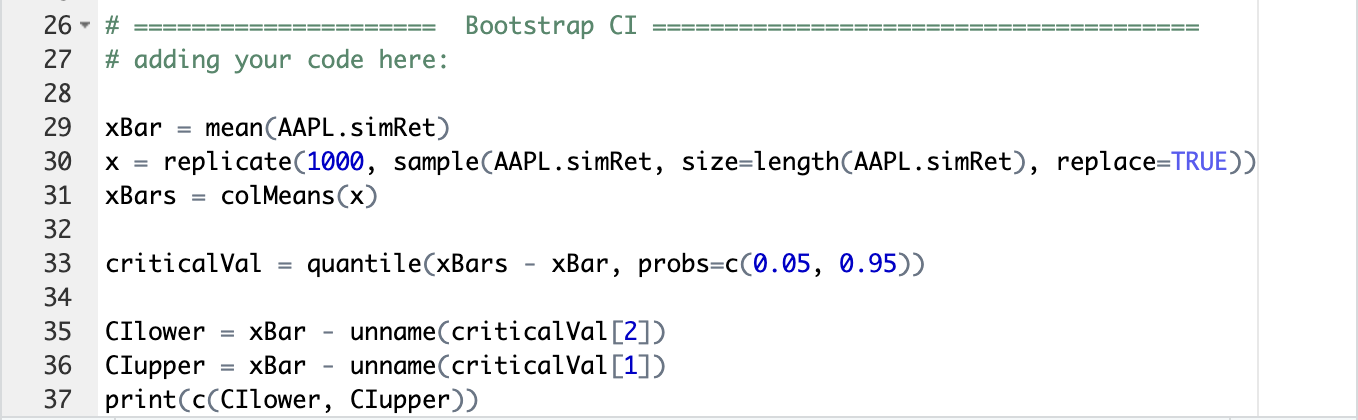
\includegraphics[scale=0.5]{script.png}
        \caption{\emph{R script for Problem 19-1.}}
    \end{figure}
    \begin{figure}[h]
        \centering
        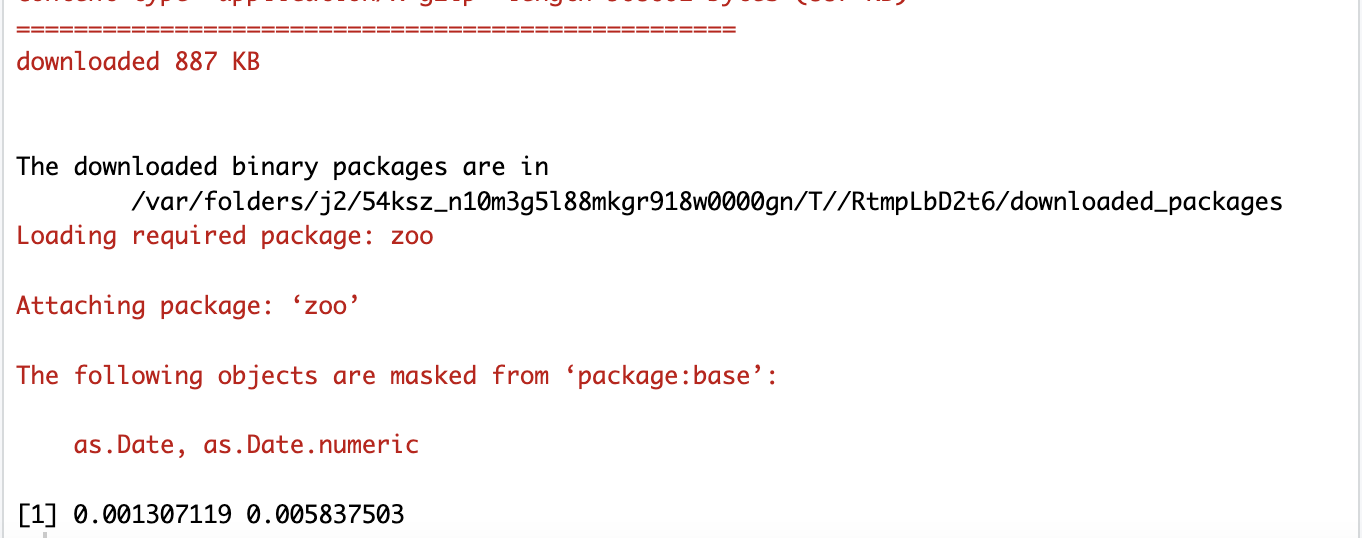
\includegraphics[scale=0.5]{result.png}
        \caption{\emph{The confidence interval is (0.00131, 0.00584).}}
    \end{figure}
\end{proof}

\newpage
\textbf{Problem 7.5.7}
Start with the fact that $(n - 1)S^2/\sigma^2$ has a chi square distribution with $n - 1$ df (if the $Y_i$'s are normally distributed) and derive the confidence interval formulas given in Theorem 7.5.1:
\begin{enumerate}[label=(\alph*)]
    \item 
    a $100(1-\alpha)\%$ confidence interval for $\sigma^2$ is the set of values $$\left(\frac{(n-1)s^2}{\chi^2_{1-\alpha/2, n-1}}, \frac{(n-1)s^2}{\chi^2_{\alpha/2, n-1}}\right).$$
    \begin{proof}[Solution]
        \begin{align*}
            P\left(\chi^2_{\alpha/2, n-1}\le \frac{(n-1)S^2}{\sigma^2} \le \chi^2_{1-\alpha/2, n-1}\right) &= 1-\alpha \\
            P\left(\frac{1}{\chi^2_{\alpha/2, n-1}}\ge \frac{\sigma^2}{(n-1)S^2} \ge \frac{1}{\chi^2_{1-\alpha/2, n-1}}\right) &= 1-\alpha \\
            P\left(\frac{(n-1)S^2}{\chi^2_{\alpha/2, n-1}}\ge \sigma^2 \ge \frac{(n-1)S^2}{\chi^2_{1-\alpha/2, n-1}}\right) &= 1-\alpha 
        \end{align*}
        Hence, we can see a $100(1-\alpha)\%$ confidence interval for $\sigma^2$ is the set of values $$\left(\frac{(n-1)s^2}{\chi^2_{1-\alpha/2, n-1}}, \frac{(n-1)s^2}{\chi^2_{\alpha/2, n-1}}\right).$$
    \end{proof}

    \item
    a $100(1-\alpha)\%$ confidence interval for $\sigma$ is the set of values $$\left(\sqrt{\frac{(n-1)s^2}{\chi^2_{1-\alpha/2, n-1}}}, \sqrt{\frac{(n-1)s^2}{\chi^2_{\alpha/2, n-1}}}\right)$$
    \begin{proof}[Solution]
        Similarly,
        \begin{align*}
            P\left(\chi^2_{\alpha/2, n-1}\le \frac{(n-1)S^2}{\sigma^2} \le \chi^2_{1-\alpha/2, n-1}\right) &= 1-\alpha \\
            P\left(\frac{1}{\chi^2_{\alpha/2, n-1}}\ge \frac{\sigma^2}{(n-1)S^2} \ge \frac{1}{\chi^2_{1-\alpha/2, n-1}}\right) &= 1-\alpha \\
            P\left(\frac{(n-1)S^2}{\chi^2_{\alpha/2, n-1}}\ge \sigma^2 \ge \frac{(n-1)S^2}{\chi^2_{1-\alpha/2, n-1}}\right) &= 1-\alpha \\
            P\left(\sqrt{\frac{(n-1)S^2}{\chi^2_{\alpha/2, n-1}}}\ge \sigma \ge \sqrt{\frac{(n-1)S^2}{\chi^2_{1-\alpha/2, n-1}}}\right) &= 1-\alpha 
        \end{align*}
        Hence, we can see a $100(1-\alpha)\%$ confidence interval for $\sigma$ is the set of values $$\left(\sqrt{\frac{(n-1)s^2}{\chi^2_{1-\alpha/2, n-1}}}, \sqrt{\frac{(n-1)s^2}{\chi^2_{\alpha/2, n-1}}}\right).$$
    \end{proof}
\end{enumerate}
\bigbreak

\newpage
\textbf{Problem 7.5.12}
\begin{enumerate}[label=(\alph*)]
    \item 
    Use the asymptotic normality of chi square random variables (see Question 7.3.6) to derive large-sample confidence interval formulas for $\sigma$ and $\sigma^2$.
    \begin{proof}[Solution]
        The asymptotic normality of chi square random variables states that:
        $$\frac{\chi^2_n - n}{\sqrt{2n}} \sim N(0,1).$$

        Then, we can write
        \begin{align*}
            \frac{\chi^2_{n-1}-(n-1)}{\sqrt{2(n-1)}} & \approx Z \\
            \chi^2_{n-1} & \approx Z\sqrt{2(n-1)}+(n-1) \\
            \chi^2_{n-1} & \sim N(n-1, 2(n-1)). \\
        \end{align*}

        Hence, we conclude as $n$ goes to infinity, $\chi^2_{n-1}$ converges to $N(n-1, 2(n-1))$.
        Then, we can find the confidence interval for $\sigma^2$ and $\sigma$ as follows:
        \begin{align*}
            P\left(Z_{\alpha/2}\sqrt{2(n-1)}+(n-1)\le \frac{(n-1)S^2}{\sigma^2} \le Z_{1-\alpha/2}\sqrt{2(n-1)}+(n-1)\right) &= 1-\alpha \\
            P\left(\frac{1}{Z_{\alpha/2}\sqrt{2(n-1)}+(n-1)}\ge \frac{\sigma^2}{(n-1)S^2} \ge \frac{1}{Z_{1-\alpha/2}\sqrt{2(n-1)}+(n-1)}\right) &= 1-\alpha \\
            P\left(\frac{(n-1)S^2}{Z_{\alpha/2}\sqrt{2(n-1)}+(n-1)}\ge \sigma^2 \ge \frac{(n-1)S^2}{Z_{1-\alpha/2}\sqrt{2(n-1)}+(n-1)}\right) &= 1-\alpha \\ 
            P\left(\sqrt{\frac{(n-1)S^2}{Z_{\alpha/2}\sqrt{2(n-1)}+(n-1)}}\ge \sigma \ge \sqrt{\frac{(n-1)S^2}{Z_{1-\alpha/2}\sqrt{2(n-1)}+(n-1)}}\right) &= 1-\alpha.
        \end{align*}
        Therefore, we can see a $100(1-\alpha)\%$ confidence interval for $\sigma^2$ is the set of values $$\left(\frac{(n-1)s^2}{Z_{1-\alpha/2}\sqrt{2(n-1)}+(n-1)}, \frac{(n-1)s^2}{Z_{\alpha/2}\sqrt{2(n-1)}+(n-1)}\right),$$
        and the $100(1-\alpha)\%$ confidence interval for $\sigma$ is the set of values $$\left(\sqrt{\frac{(n-1)s^2}{Z_{1-\alpha/2}\sqrt{2(n-1)}+(n-1)}}, \sqrt{\frac{(n-1)s^2}{Z_{\alpha/2}\sqrt{2(n-1)}+(n-1)}}\right).$$
    \end{proof}
    
    \newpage
    \item
    Use your answer to part (a) to construct an approximate 95\% confidence interval for the standard deviation of estimated potassium-argon ages based on the nineteen $y_i$'s in Table 7.5.1. 
    How does this confidence interval compare with the one in Case Study 7.5.1: (20.5 million years, 40.0 million years)?
    \begin{displaymath}
        \begin{array}{|c|c|}
            \hline
            \emph{Specimen} & \emph{Estimated Age (millions of years)} \\
            \hline
            1 & 249 \\
            2 & 254 \\
            3 & 243 \\
            4 & 268 \\
            5 & 253 \\
            6 & 269 \\
            7 & 287 \\
            8 & 241 \\ 
            9 & 273 \\
            10 & 306 \\
            11 & 303 \\
            12 & 280 \\
            13 & 260 \\
            14 & 256 \\
            15 & 278 \\
            16 & 344 \\
            17 & 304 \\
            18 & 283 \\
            19 & 310 \\            
            \hline
        \end{array}
    \end{displaymath}
    \begin{proof}[Solution]
        \begin{align*}
            s^2 & = 733.47 \\
            \sigma & \in \left(\sqrt{\frac{18\times 733.47}{1.96\sqrt{2\times 18}+18}}, \sqrt{\frac{18\times 733.47}{-1.96\sqrt{2\times 18}+18}}\right) \\
            & \in (21.06, 45.99)
        \end{align*}
        The confidence interval is approximately the same as the one in Case Study 7.5.1.
    \end{proof}
\end{enumerate}
\end{document}
